\documentclass{beamer}
\usetheme{CERN}

\usepackage{amsfonts,amsmath,oldgerm,algorithmic,algorithm} % Math packages

\usepackage{tikz} % Tikz package for drawing 
\usetikzlibrary{calc}
\usetikzlibrary{shapes.callouts}

% \usepackage{pdfpages} % For including pdf files
\usepackage{geometry}

% TODO: For including code snippets
% \usepackage{listings}
% \usepackage{minted}

\usepackage{hyperref}
\hypersetup{%
  colorlinks=false,% hyperlinks will be black
  urlbordercolor = black,
  % linkbordercolor=red,% hyperlink borders will be red
  pdfborderstyle={/S/U/W 1}% border style will be underline of width 1pt
}

% For Tables and Figures
\usepackage{booktabs}
\usepackage{multirow}
\usepackage{caption} 
\captionsetup{font=tiny,labelfont=bf,skip=0pt, justification=centering}
\usepackage{subcaption}
\usepackage{float}



\usepackage[append]{beamersubframe}

% \beamertemplategridbackground[1cm]
\setbeamersize
{
    text margin left=1cm,
    text margin right=1cm
}

\AtBeginSection[]{
  \begin{frame}
  \vfill
  \centering
  \begin{beamercolorbox}[sep=8pt,center,shadow=false,rounded=false]{title}
    \usebeamerfont{title}\insertsectionhead\par%
  \end{beamercolorbox}
  \vfill
  \end{frame}
}



\title{Work Summary}
\subtitle{Liverpool FASER Meeting}
\date{February 7, 2025}
\author{Pawan Johnson}
\institute{University of Liverpool}
% \date{\today}


\begin{document}

\begingroup
\setbeamertemplate{footline}{}
\begin{frame}
    \maketitle
\end{frame}
\endgroup

% \begin{frame}
%     \frametitle{Introduction}
%     \begin{itemize}
%         \item Hello, I am Pawan!
%     \end{itemize}
% \end{frame}

\begin{frame}{My work thus far ...}
    \begin{itemize}
        \item 2024 DQ Checks for Tracking Variables
        \begin{itemize}
            \item Presented at Physics General Meeting on 17 December 
            \item \href{https://indico.cern.ch/event/1488927/contributions/6275978/attachments/2988614/5264126/main.pdf}{Link to Slides}
        \end{itemize}
        \item Followup to the 2024 DQ Checks
        \begin{itemize}
            \item Almost finished up with the underlying work 
            \item Writing up the slides
            \item Hoping to send out early next week
        \end{itemize}
        \item Working on ALMA9 Efficiency Checks for DP
        \begin{itemize}
            \item Almost finished up 
            \item Hoping to present on Monday
        \end{itemize}
    \end{itemize}
\end{frame}



\begin{frame}{2024 DQ Checks}
    \begin{itemize}
        \item Look at all of 2024 Data and compare it to 2023
        \item Focus was on the Track Variables
        \item Expected good agreements?
        \item But agreements weren't straightforward
        \begin{itemize}
            \item Variables like Positions were fine.
            \item Momenta were not
            \item Most variables were quite different
            \item Attributed to the changed background and changed optics
            \item Made one to one correspondence with 2023 data difficult
        \end{itemize}
    \end{itemize}
\end{frame}

\begin{frame}{2024 DQ Checks -- Some Plots}
    \begin{itemize}
        \item We knew the beam crossing angle changed 
        \item From -160 $\mu$rad in 2023 to +160 $\mu$rad in 2024 
    \end{itemize}
    \begin{columns}
        \begin{column}{0.5 \textwidth}
            \begin{figure}
                \centering
                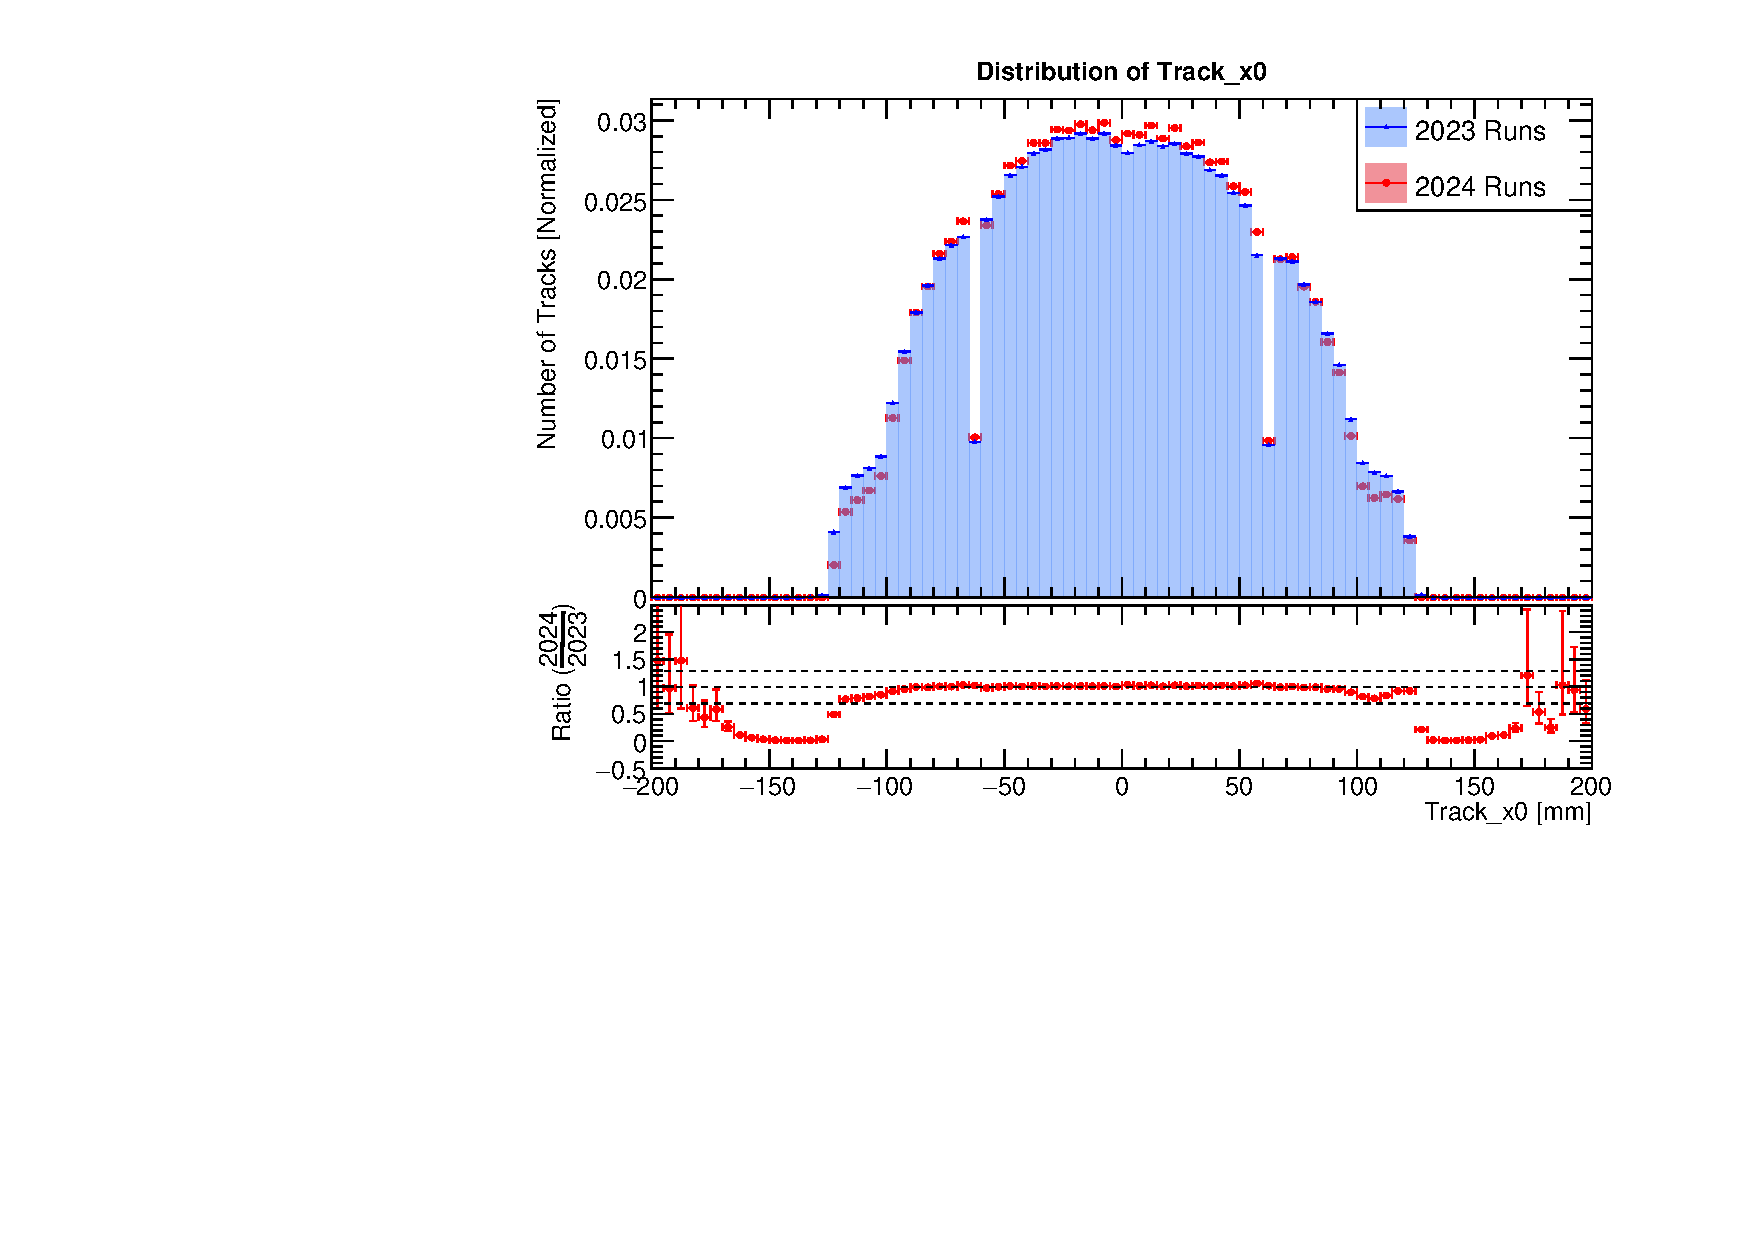
\includegraphics[width=\textwidth]{assets/Track_x0.pdf}
                \caption{Track x0}
            \end{figure}
        \end{column}
        \begin{column}{0.5 \textwidth}
            \begin{figure}
                \centering
                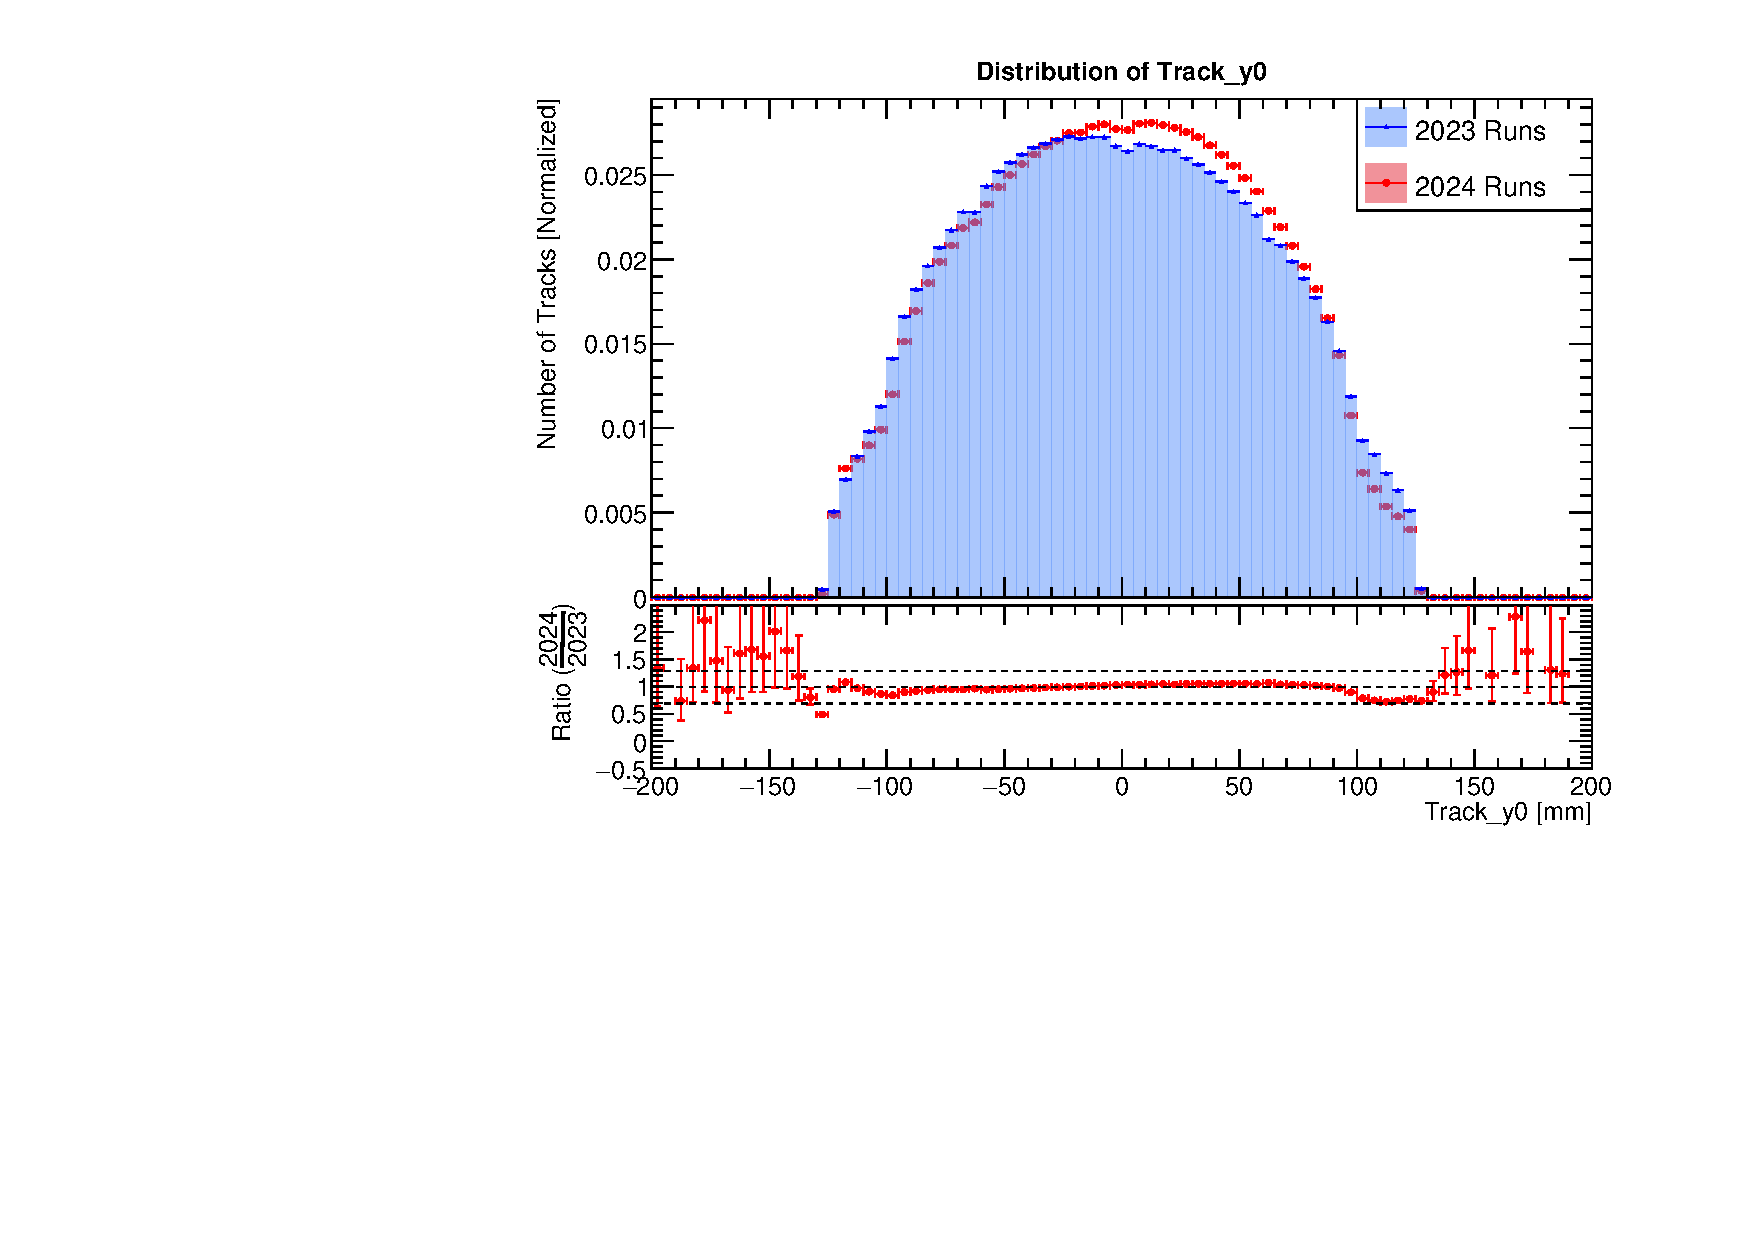
\includegraphics[width=\textwidth]{assets/Track_y0.pdf}
                \caption{Track y0}
            \end{figure}
        \end{column}
    \end{columns}
    \begin{itemize}
        \item We observed the corresponding shift in the the track positions
    \end{itemize}
\end{frame}

\begin{frame}{2024 DQ Checks -- Some Plots}
    \begin{itemize}
        \item That had huge implications on the observed background
    \end{itemize}

        \begin{figure}
            \centering
            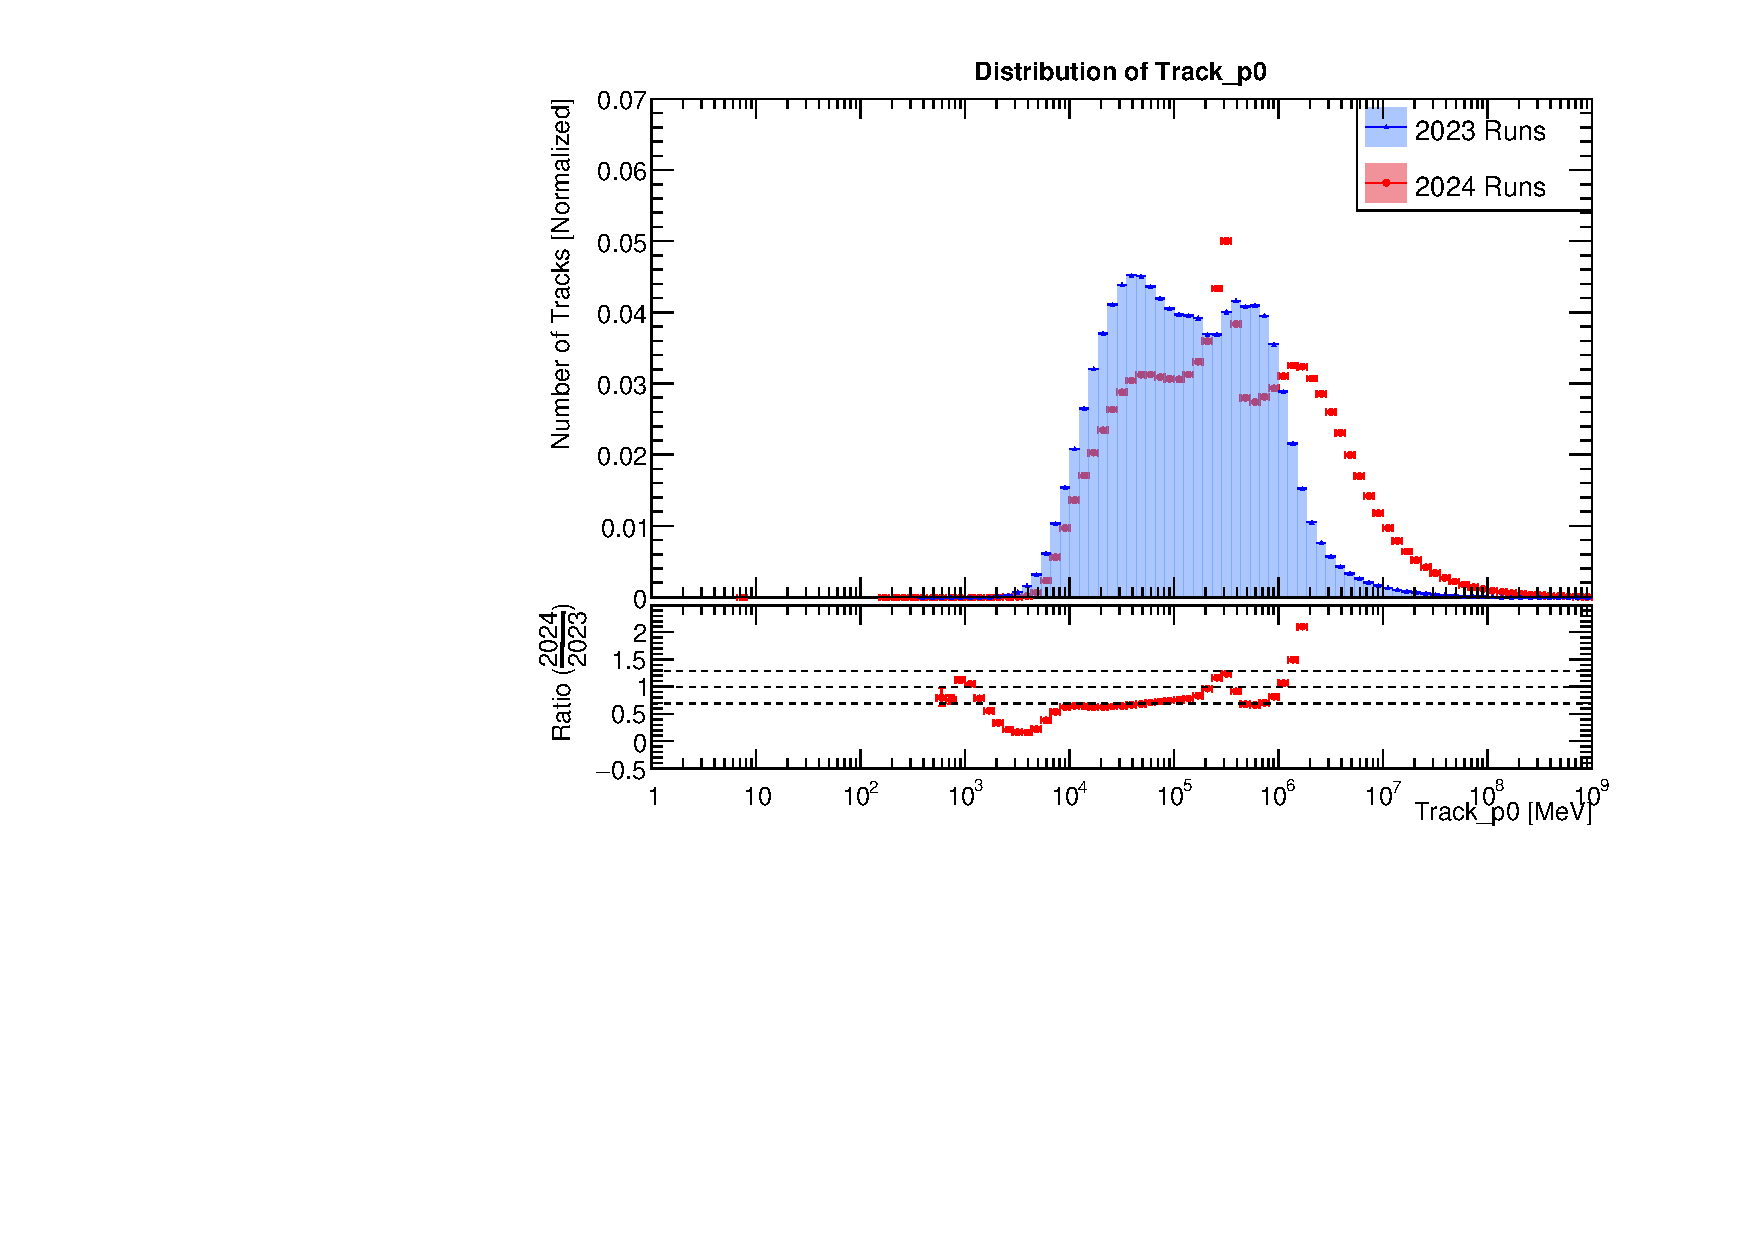
\includegraphics[width=0.7\textwidth]{assets/Track_p0.pdf}
            \caption{Track p0}
        \end{figure}
    \begin{itemize}
        \item Lot more high-momenta-positively charged muons in 2024
        \item This had non-trivial effects on the other track parameters
    \end{itemize}
\end{frame}

% \begin{frame}{Assimilate Comments from the Email}
%     \begin{itemize}
%         \item Do momenta binning for have a more equitable correspondence between 2023 and 2024
%         \item 
%     \end{itemize}
% \end{frame}

\begin{frame}{Follow Up on 2024 DQ Checks}
    \begin{itemize}
        \item Do a momentum binning to see if we can have a more equitable correspondence between 2023 and 2024
        \item Some new variables were introduced in the 2024 data
        \begin{itemize}
            \item module\_eta0, module\_phi0 
            \item which describes the first tracking module hit by the track
        \end{itemize}
    \item Start looking at the track parameters as a function of the starting module of the track
    \item Also needed updates to the 2024 runlist [Preliminary]
    \item Updates to the Yield Plots 
    \item Comparative analysis between four run periods in 2024
    \item Should be sent out early next week
    \end{itemize}
\end{frame}


\begin{frame}{2024 DQ Followup -- Some Plots}
\begin{columns}
    \begin{column}{0.7 \textwidth}
        \begin{figure}
            \centering
            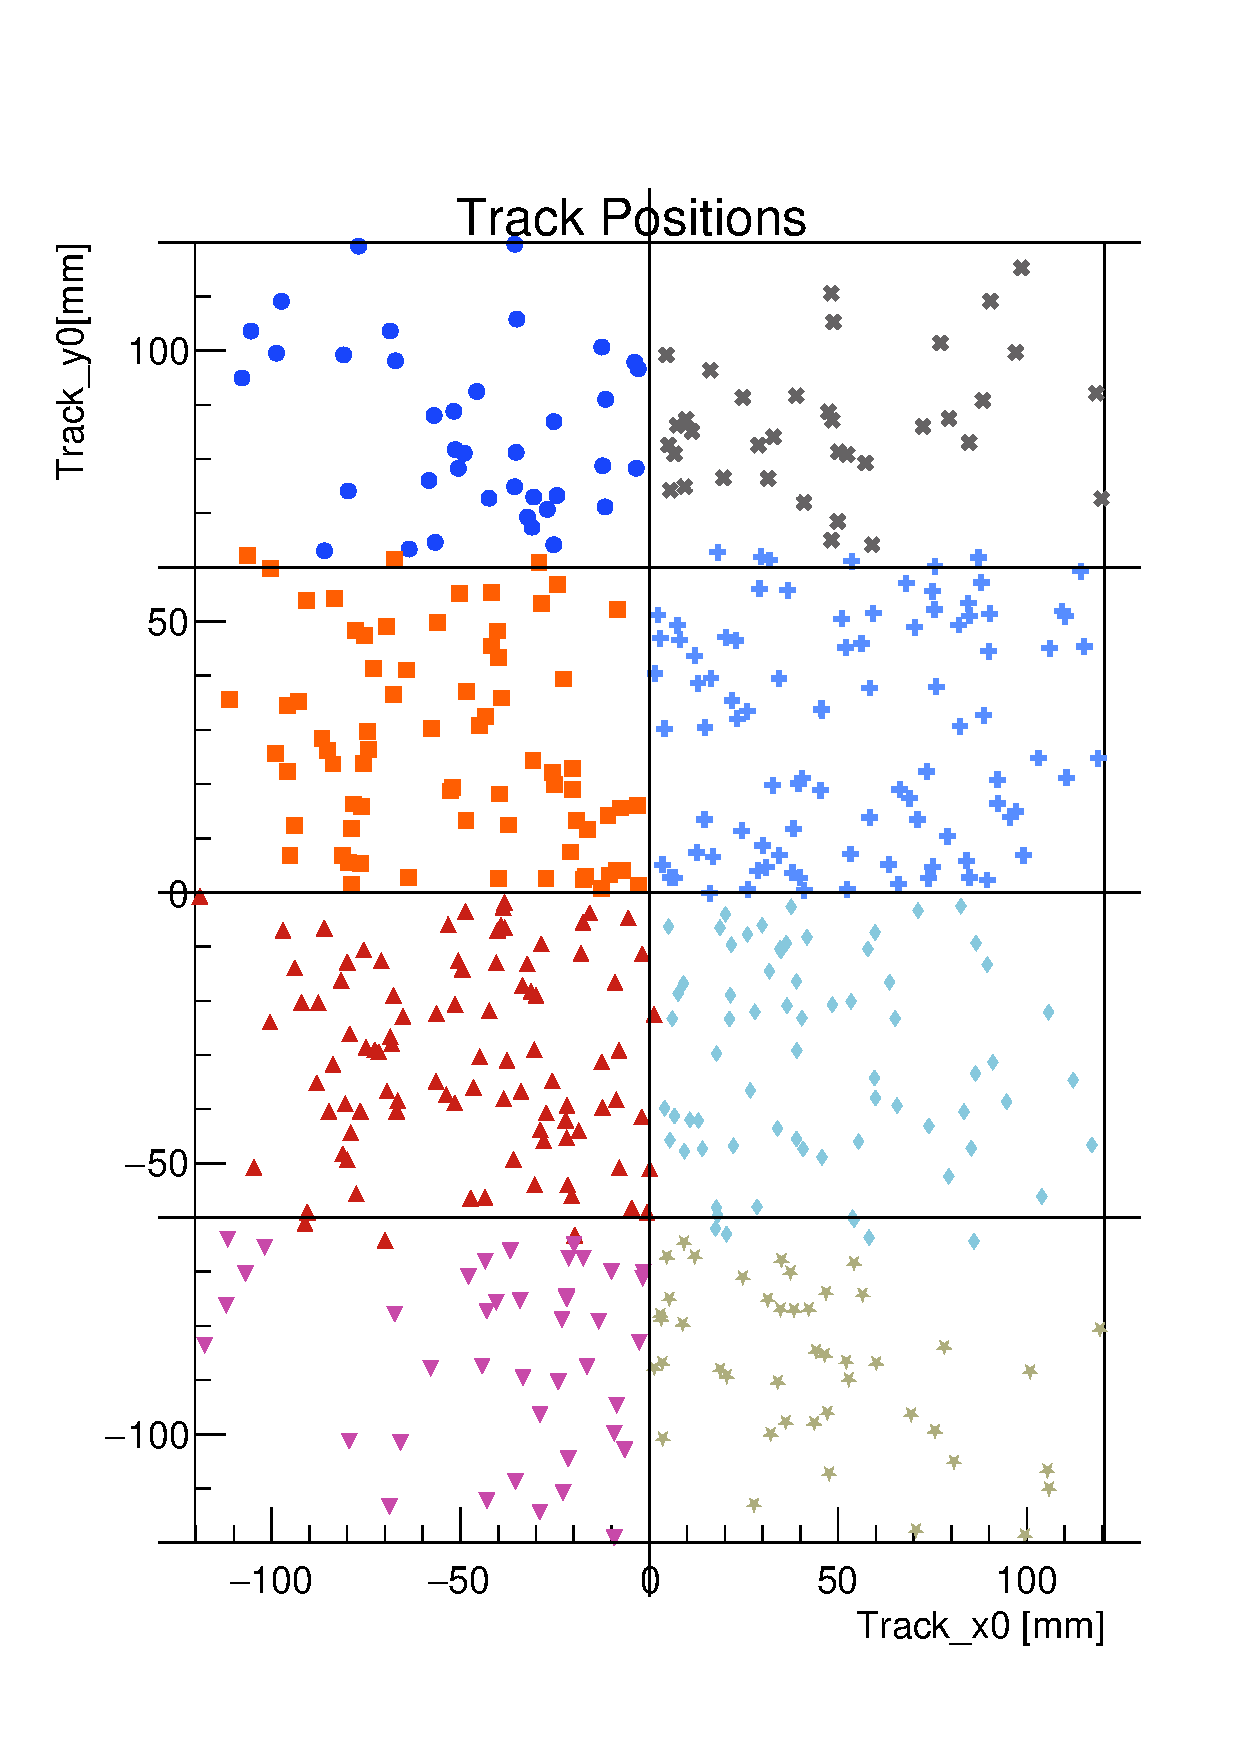
\includegraphics[height=0.7\textheight]{assets/Positions_st0_truemodule0.pdf}
            \caption{Track Points across Module}
        \end{figure}
    \end{column}
    \hspace{-2cm}\begin{column}{0.6 \textwidth}
        \begin{figure}
            \centering
            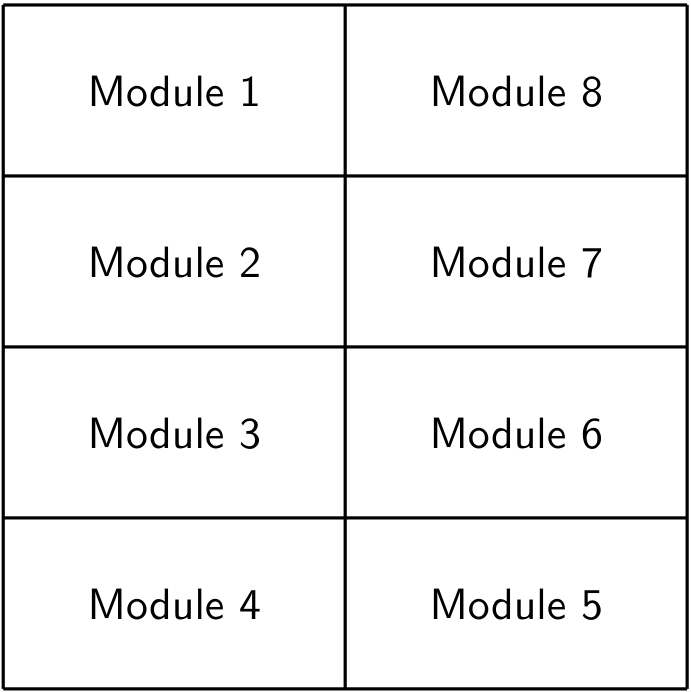
\includegraphics[height=0.4\textwidth]{assets/ModuleThumbnail.png}
            \caption{Module Numbering}
        \end{figure}
        \begin{itemize}
            \scriptsize
            \item Four central modules : 2,7,3,6
            \item Four outer modules : 1,8,4,7
        \end{itemize}
    \end{column}
\end{columns}
\end{frame}

\begin{frame}{2024 DQ Followup -- Some Plots}
    \begin{itemize}
        \item Wanted to see where the end module of the track
    \end{itemize}
    \begin{columns}
        \begin{column}{0.5\linewidth}
            \begin{figure}
                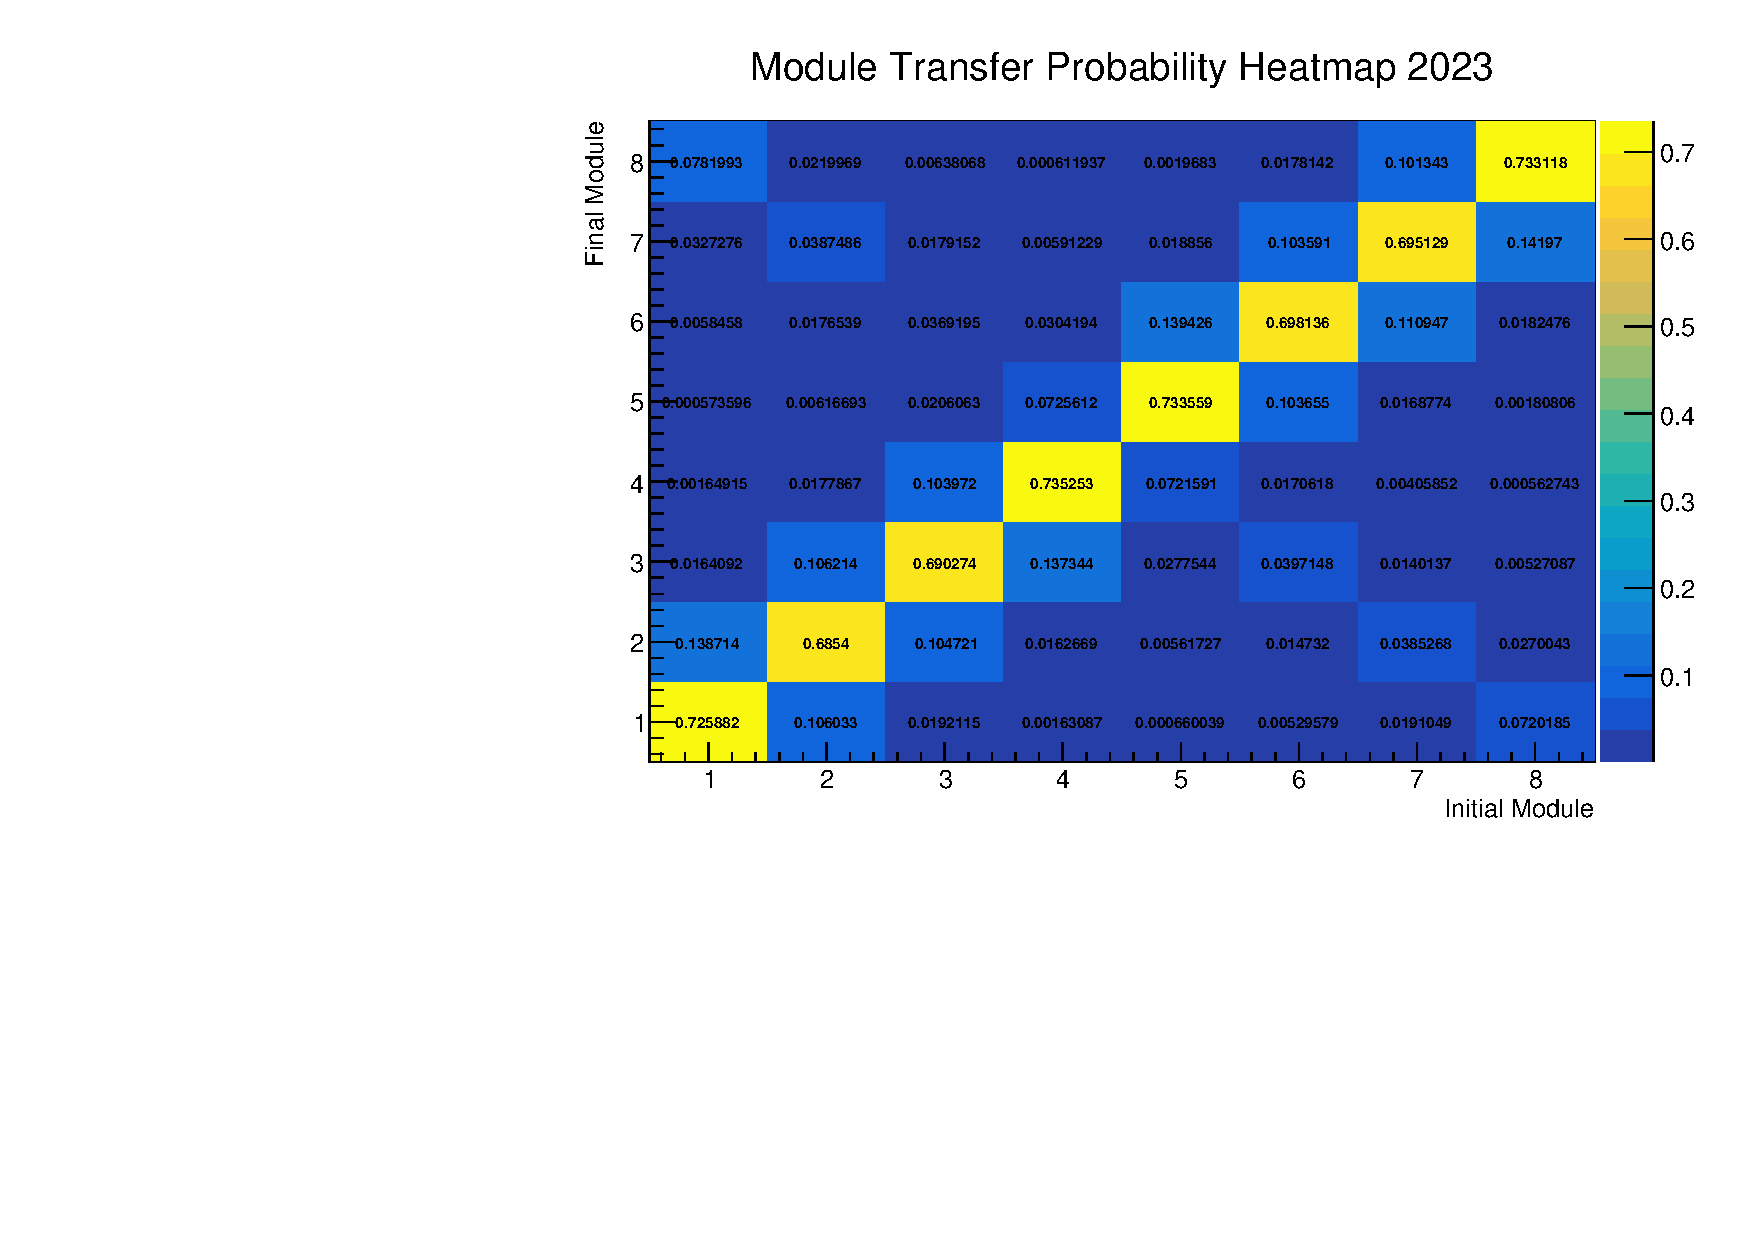
\includegraphics[width=\linewidth]{assets/st0_module_number vs st1_module_number_prob_2023.pdf}
                \caption{Probability of Transfer to a final module given a starting module [2023 data]}
            \end{figure}
        \end{column}
        \begin{column}{0.5\linewidth}
            \begin{figure}
                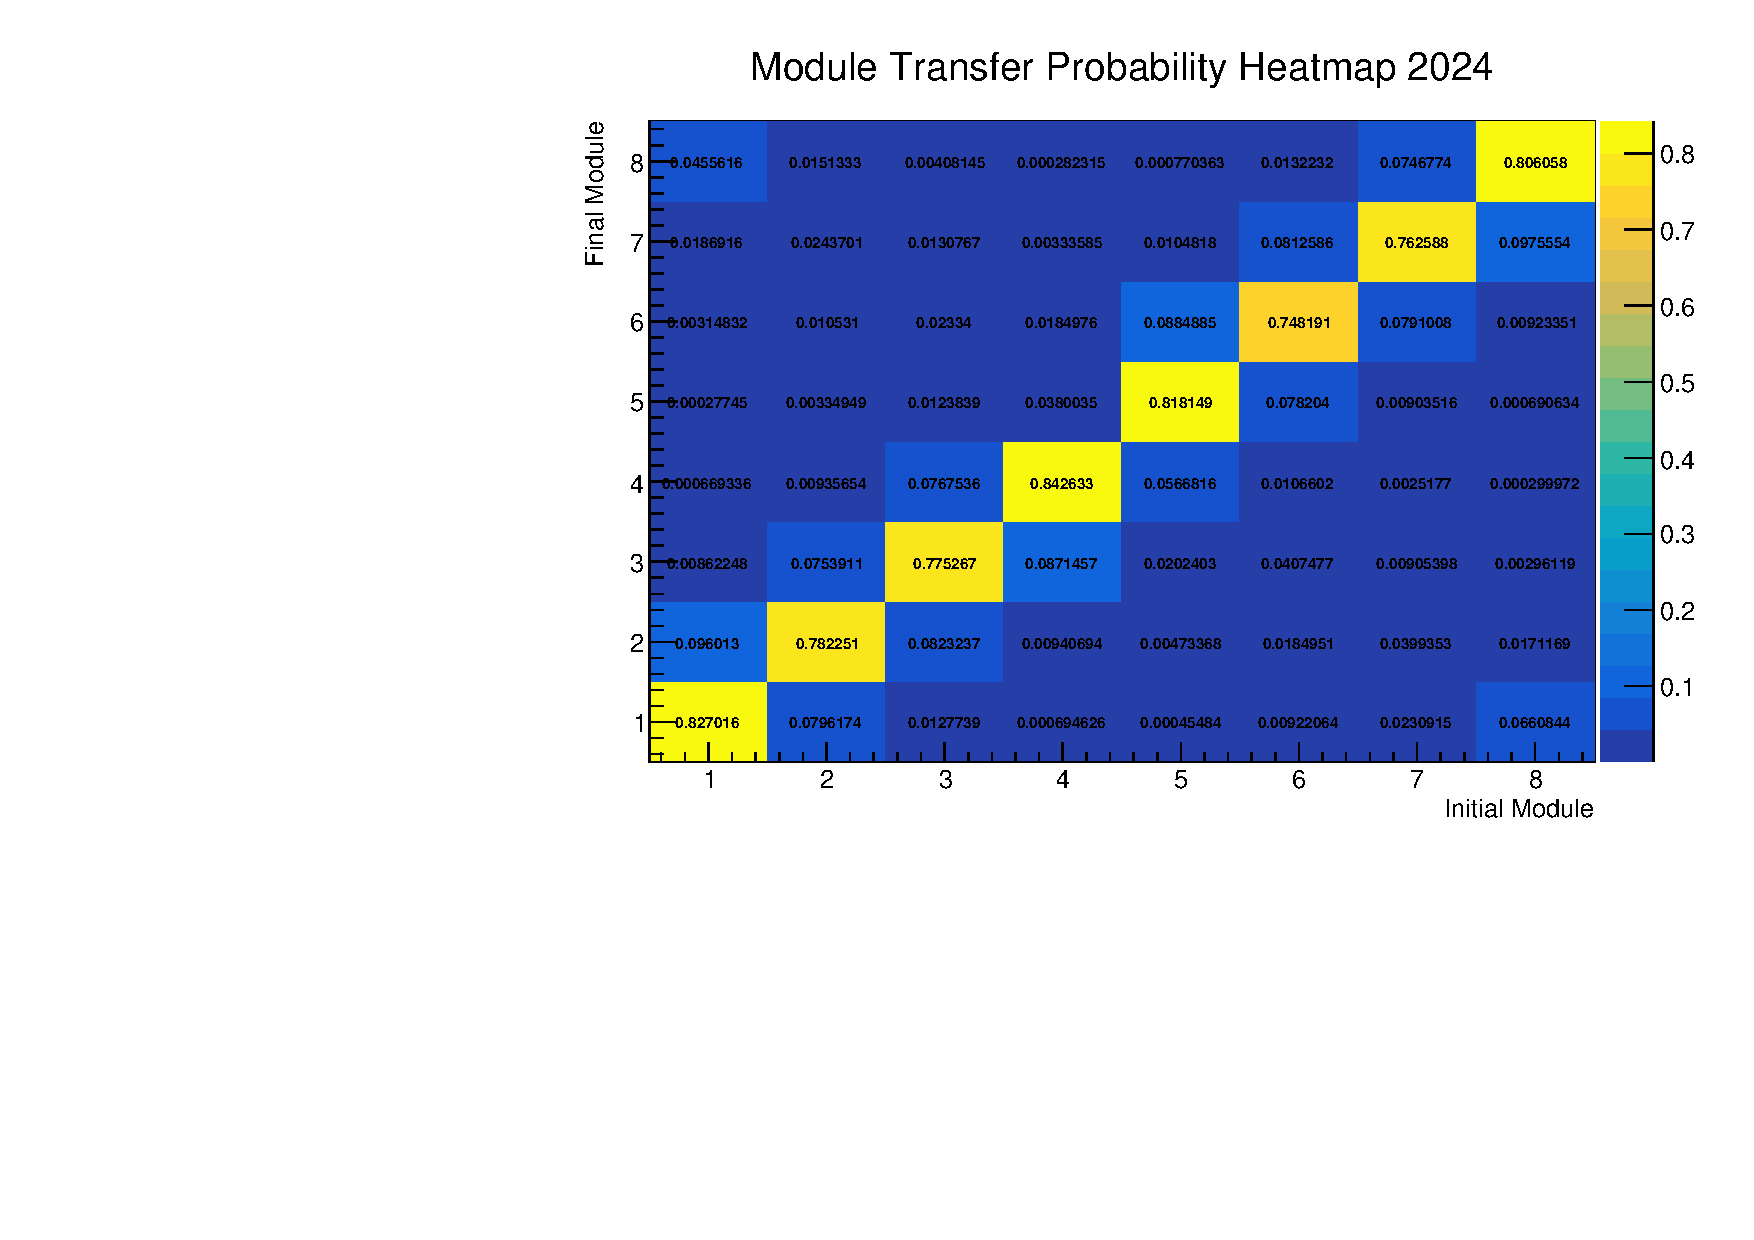
\includegraphics[width=\linewidth]{assets/st0_module_number vs st1_module_number_prob_2024.pdf}
                \caption{Probability of Transfer to a final module given a starting module [2024 data]}
            \end{figure}
        \end{column}
    \end{columns}
    \begin{itemize}
        \item We mostly transfer to the same final module 
        \begin{itemize}
            \item Some transfers to the module  top/below
            \item Some transfers to module on left/right (diagonal line)
        \end{itemize}
    \end{itemize}
\end{frame}


\begin{frame}{2024 DQ Followup -- Some Plots}
    \begin{figure}
        \centering
        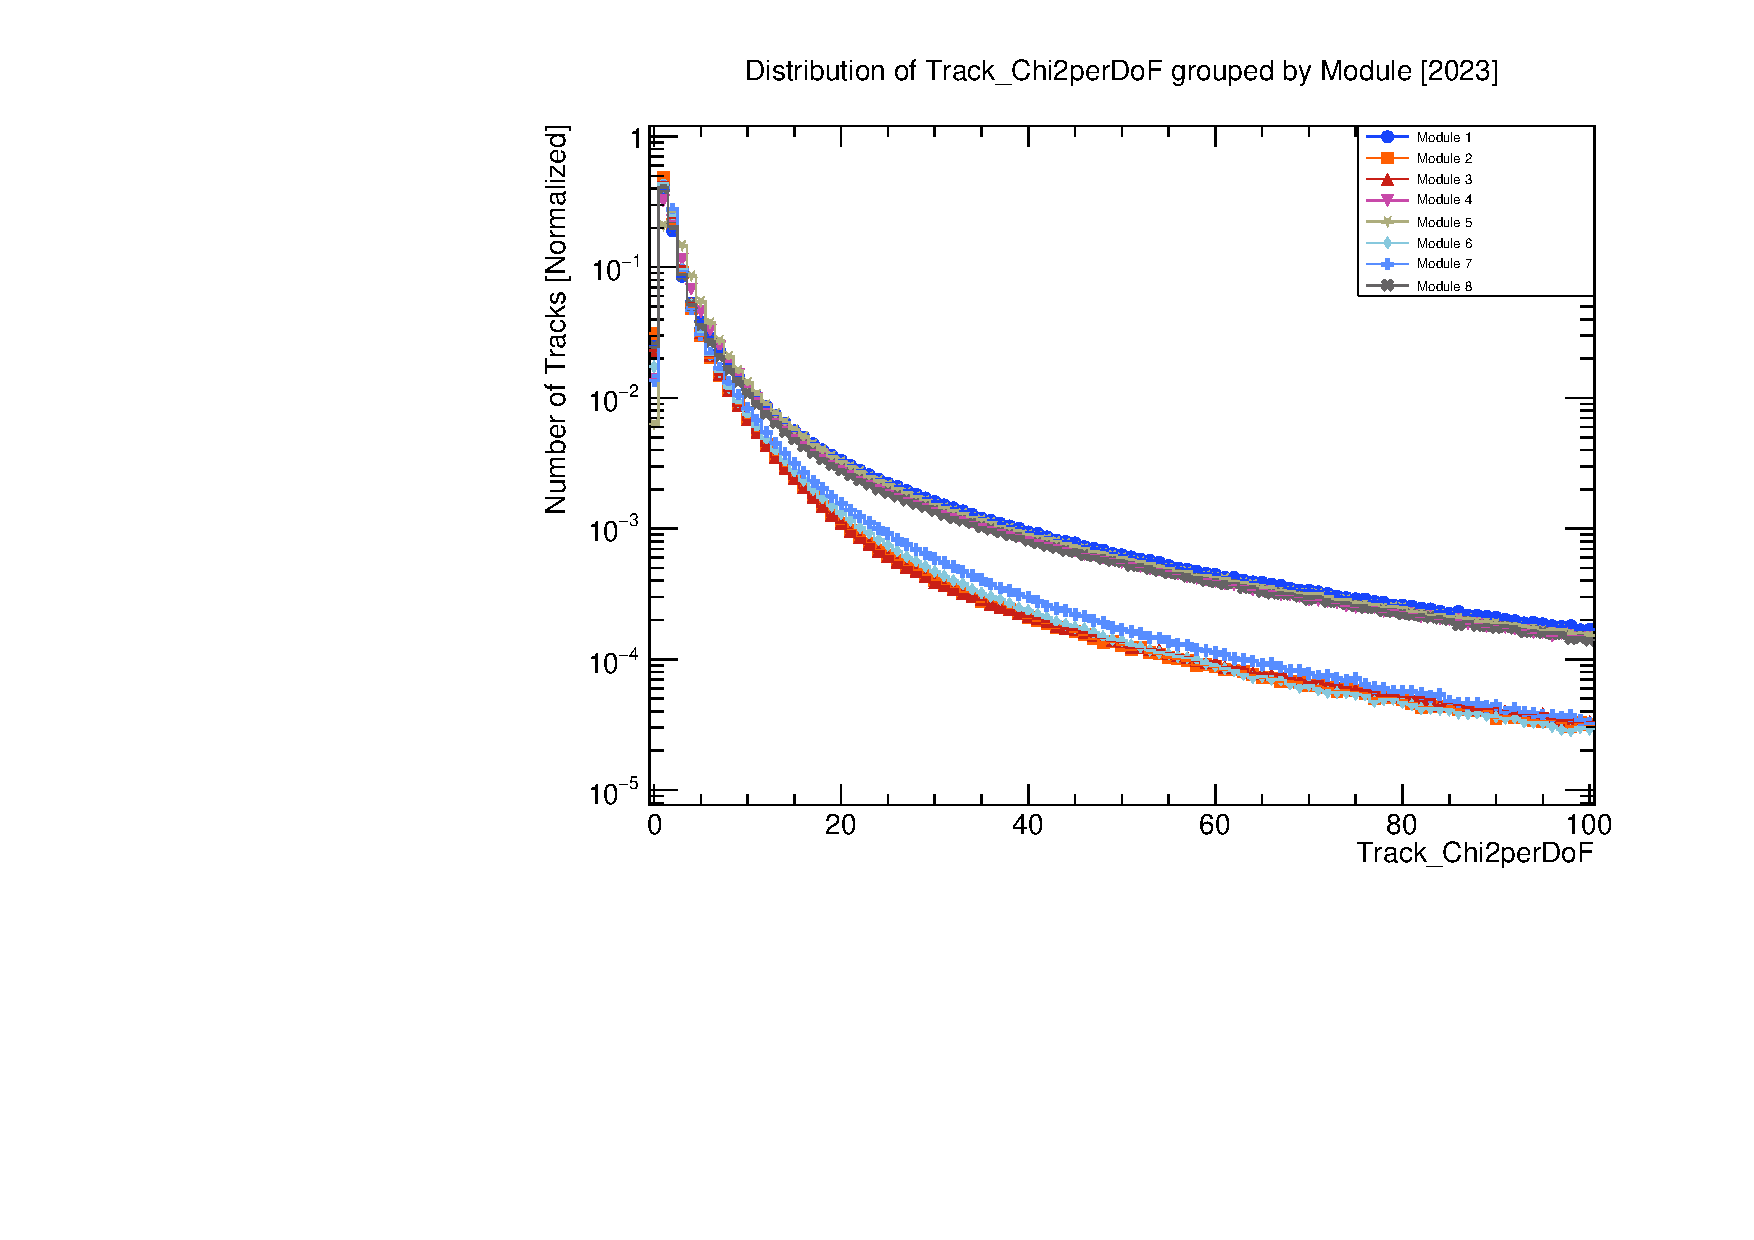
\includegraphics[width=0.7\textwidth]{assets/Track_Chi2perDoF_st0_2023.pdf}
        \caption{Track Points across Module}
    \end{figure}
    \begin{itemize}
        \item Some of the parameters factor out nicely with the central/outer module definition
    \end{itemize}
\end{frame}

\begin{frame}{Track Reconstruction Efficiency for ALMA9}
    \begin{itemize}
        \small
        \item The ALMA9 release came with updates to the track reconstruction
        \item Objective is to validate the track reconstruction for Dark Photon samples in ALMA9.
        \item Dark Photon samples have closely separated tracks making reconstruction difficult.
        \item Idea is to see if ALMA9 ``performs'' better than CENTOS7 
        \item Sinead already worked out the studies on single muon 
        \item Ansh started to look at the Analysis Cutflows
        \item Hoping to present on Monday in the Offline Software Meeting
    \end{itemize}
\end{frame}


\begin{frame}{DarkPhoton Tracking CutFlow}
    \begin{table}[h]
        \centering
        \resizebox{\linewidth}{!}{ 
            \begin{tabular}{lccccccccc}
                \toprule
                \multirow{2}{*}{Selection} & \multicolumn{4}{c}{ALMA9} & \multicolumn{4}{c}{CENTOS7} & \multirow{2}{*}{$\Delta$Eff.} \\
                \cmidrule(lr){2-5} \cmidrule(lr){6-9}
                & Pass & All & Eff. & Cum. Eff.
                & Pass & All & Eff. & Cum. Eff. \\
                \midrule
                $\geq$1 LongTracks & 56989 & 60000 & 94.98 & 94.98  & 56002 & 60000 & 93.34 & 93.34 & 1.64 \\
                $\geq$2 LongTracks & 46416 & 56989 & 81.45 & 77.36  & 45210 & 56002 & 80.73 & 75.35 & 0.72 \\
                 =2 LongTracks & 37807 & 46416 & 81.45 & 63.01  & 36746 & 45210 & 81.28 & 61.24 & 0.17 \\
                 \textcolor{red}{\textbf{Opposite Charge}} & 32427 & 37807 & 85.77 & 54.04  & 30375 & 36746 & 82.66 & 50.62 & \textcolor{red}{\textbf{3.11}}\\
                MaxRadius $<$ 100 & 31489 & 32427 & 97.11 & 52.48  & 29520 & 30375 & 97.19 & 49.20 & -0.08 \\
                \midrule
                \multicolumn{10}{c}{goodTrack Cuts}\\
                \midrule
                $\geq$ 7 Layers & 31435 & 31489 & 99.83  & 52.39  & 29472 & 29520 & 99.84  & 49.12 & -0.01 \\
                \textcolor{red}{\textbf{$\chi^2$/DoF $<$ 25}} & 31121 & 31435 & 99.00  & 51.87  & 27710 & 29472 & 94.02  & 46.18& \textcolor{red}{\textbf{4.98}} \\
                $\geq$ 7 DoF & 31115 & 31121 & 99.98  & 51.86    & 27706 & 27710 & 99.99  & 46.18 & -0.01\\
                \bottomrule
            \end{tabular}
        }
        \caption{Comparison of efficiency and cumulative efficiency for ALMA9 and CENTOS7.\\Note: The Cutflow is at an Event Level (not track level), thus the conditions have to met by all tracks in the event.}
        \label{tab:efficiency_comparison}
    \end{table}
    \begin{itemize}
        \scriptsize
        \item Highest improvement in goodTrack Cut of $\chi^2$/DoF $<$ 25
        \item Better ChargeID in ALMA9?
    \end{itemize}    
\end{frame}

\begin{frame}{Track Efficiency for ALMA9  -- Some Plots}
    \begin{itemize}
        \item Had an existing overlay study on Track Reconstruction 
    \end{itemize}
    \vspace{-0.5cm}
    \begin{columns}
        \begin{column}{0.5 \textwidth}
            \begin{figure}
                \centering
                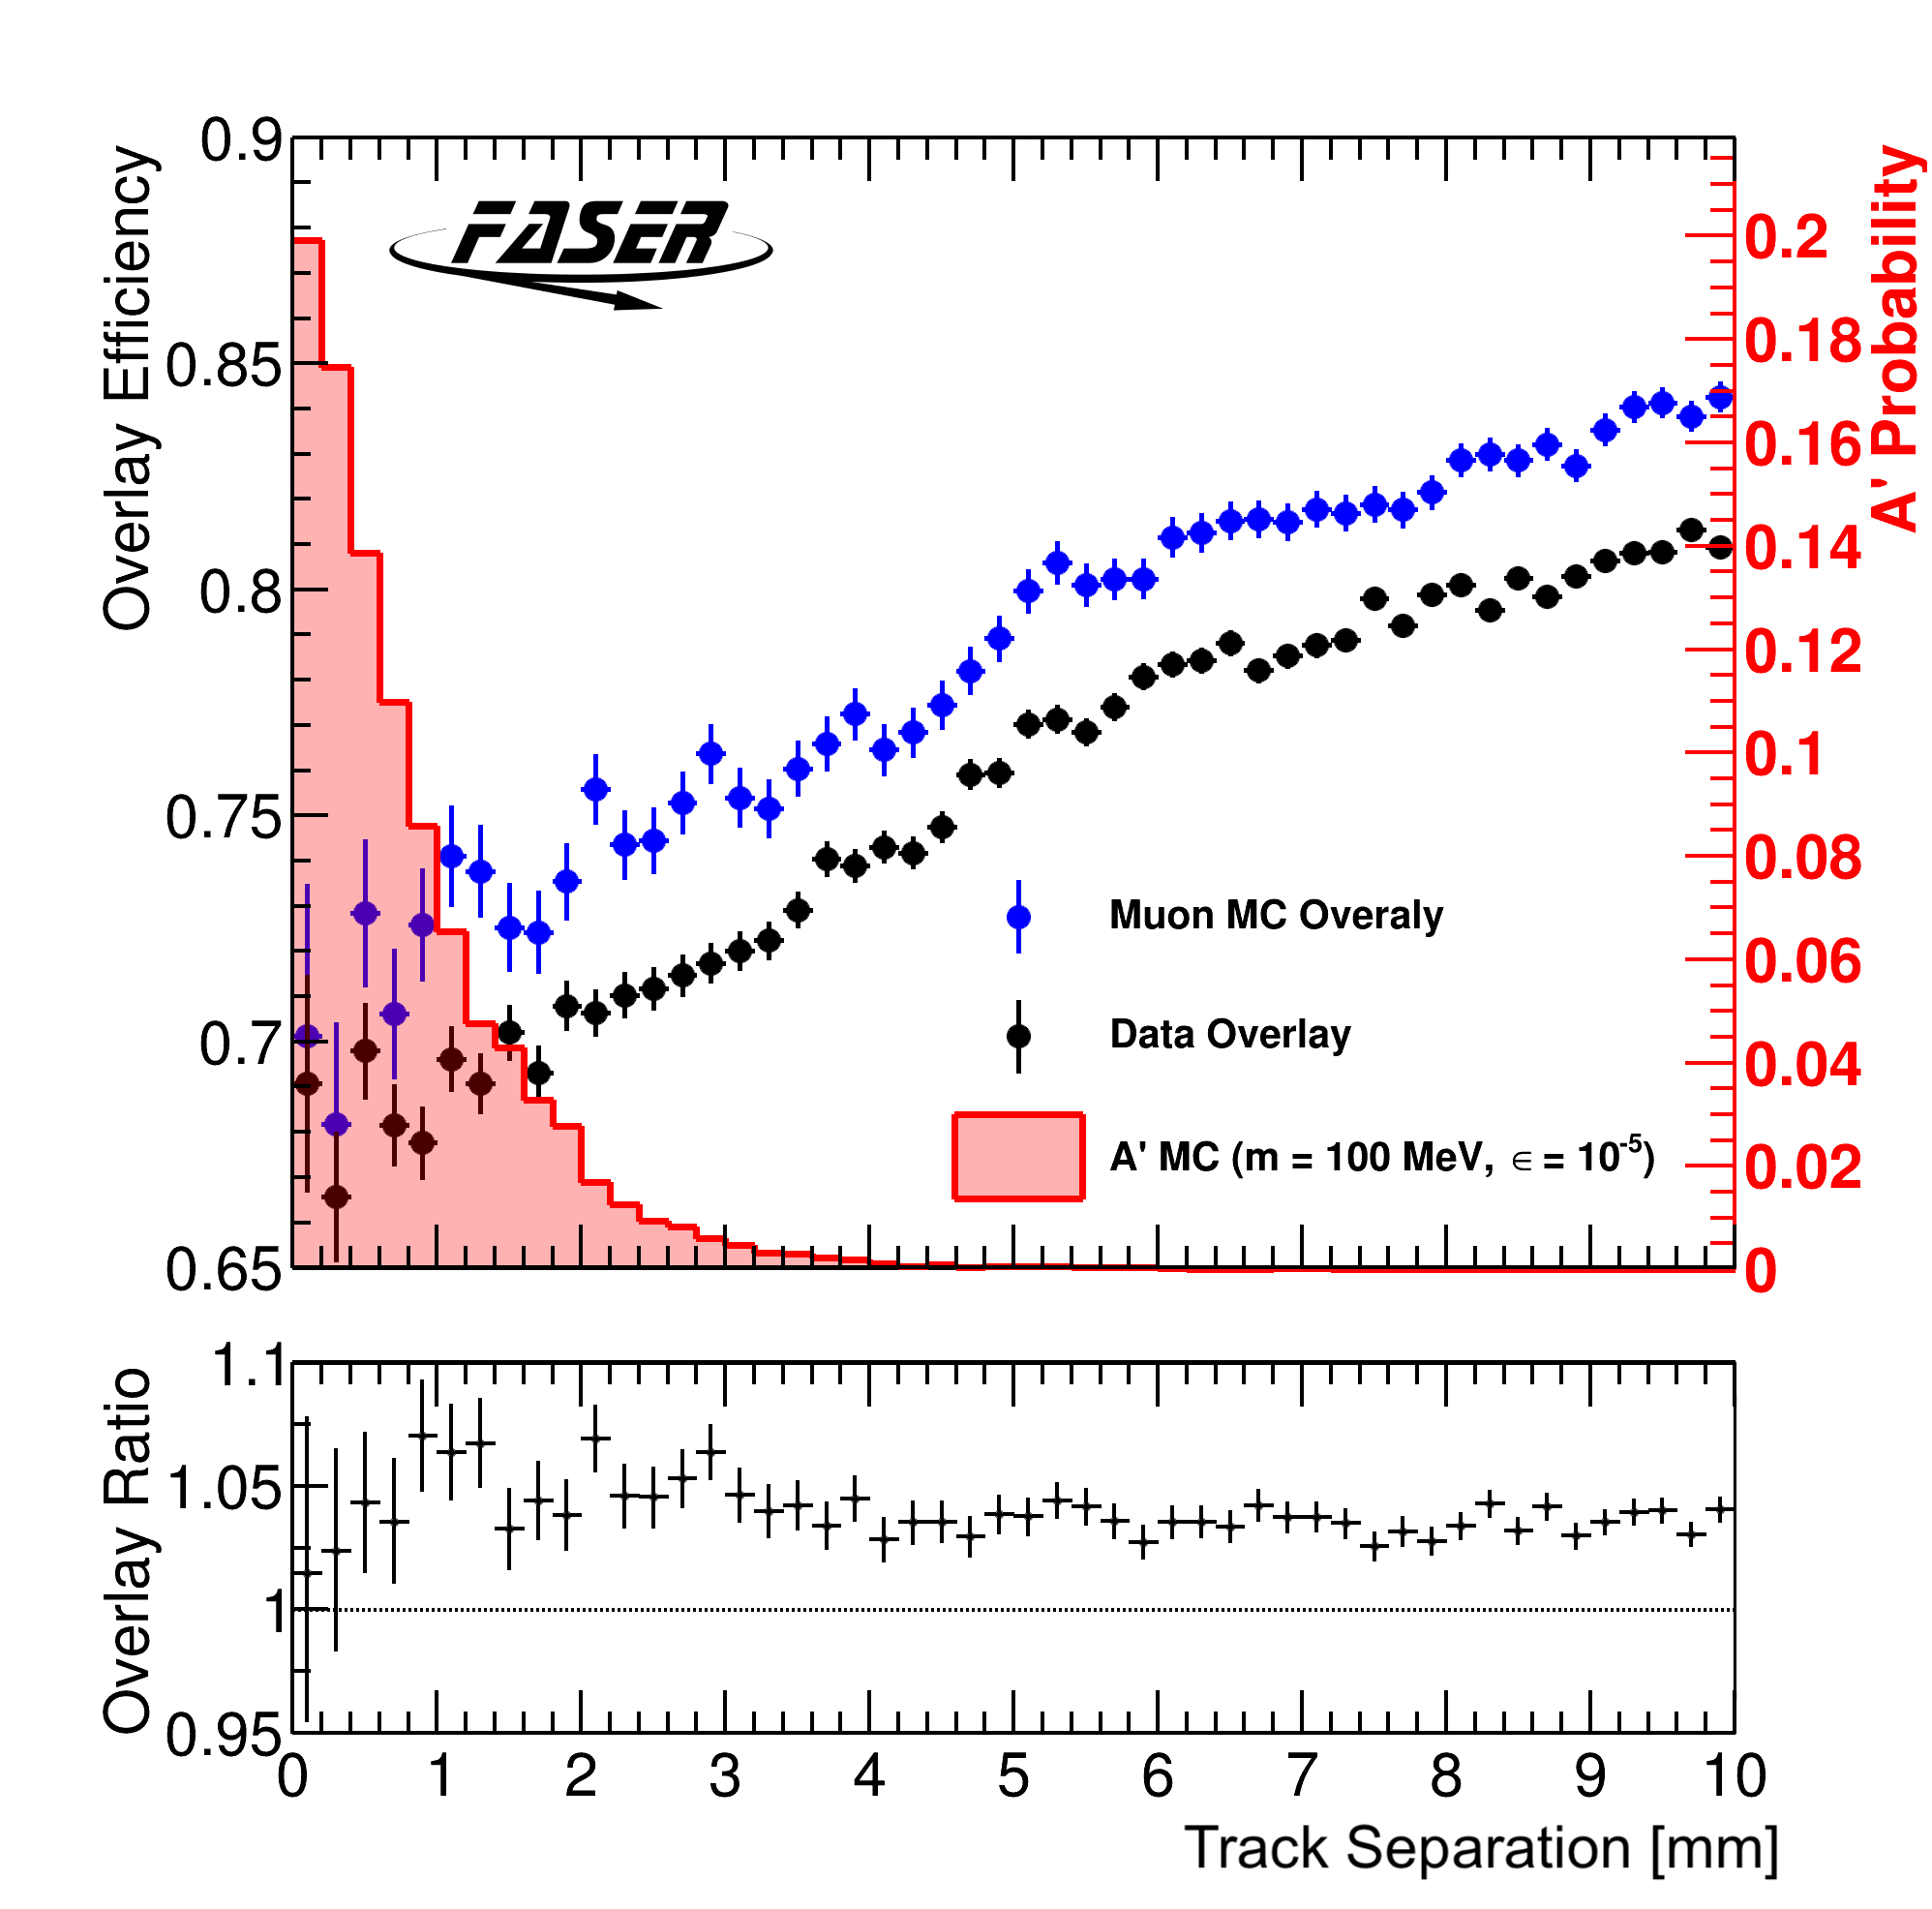
\includegraphics[width=0.8\textwidth]{assets/OverlayTracks.png}
                \caption{Overlay plot from Dark Photon Analysis}
            \end{figure}
        \end{column}
        \begin{column}{0.5 \textwidth}
            \begin{figure}
                \centering
                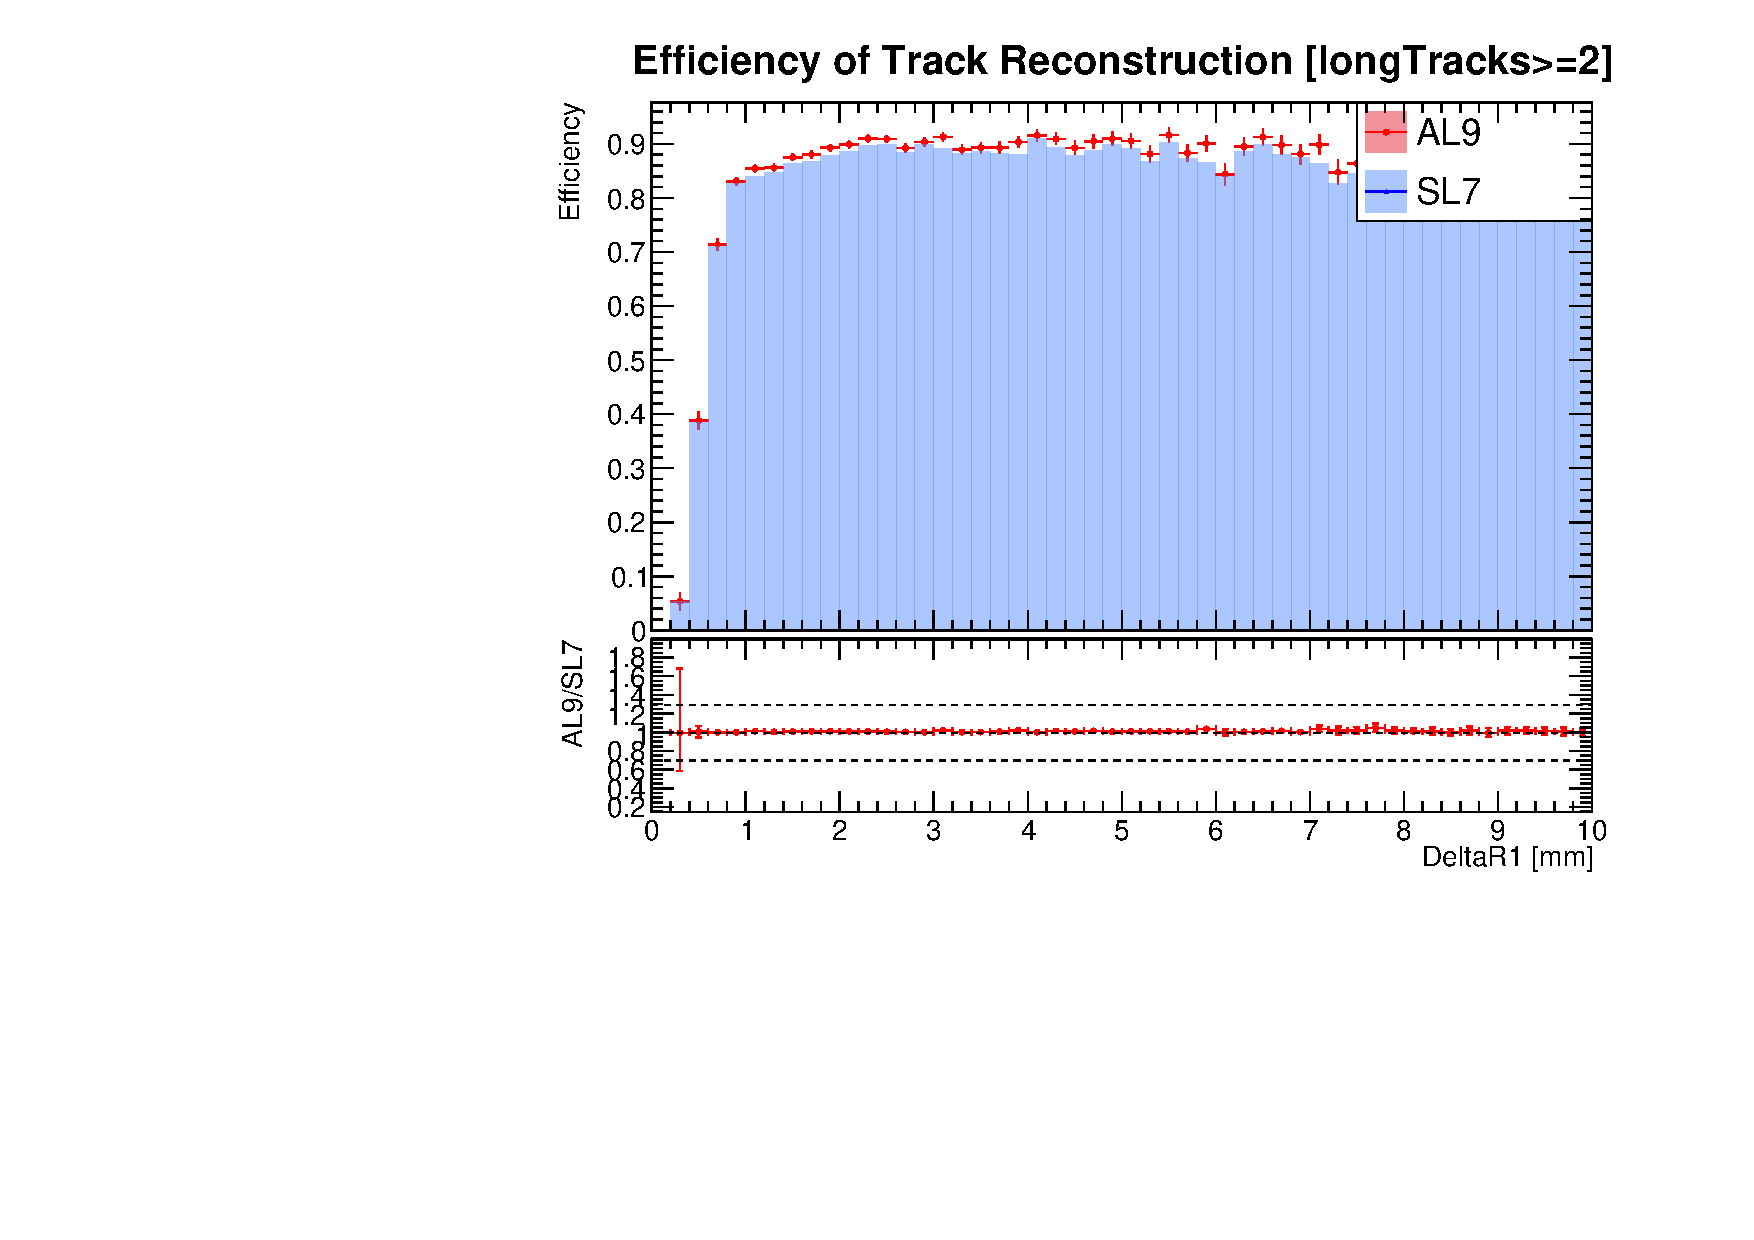
\includegraphics[width=1.1\textwidth]{assets/NEffi_greq2_DeltaR1.pdf}
                \caption{Track Efficiency ($\geq$2) as a function of distance between the tracks at the final station}
            \end{figure}
        \end{column}
    \end{columns}
    \begin{itemize}
        \item Discrepancy  with overlay studies
        \item But at least good agreement between ALMA9 and CENTOS7
        % \item Hopefully,
    \end{itemize}
\end{frame}
\begin{frame}{Work to start on}
    \begin{itemize}
        \item Start on FASER Monte Carlo Production 
        \begin{itemize}
            \item Read up on Twiki [Add Link]
            \item Possibly get involved with John?
        \end{itemize}
        \item Extended Dark Photon Search
        \begin{itemize}
            \item Develop selection for $\mu^+ \mu^-$
            \item Develop selection for $\pi^+ \pi^-$
            \item Waiting on the samples from Eric
            \item Can be done as an exercise for earlier work. 
        \end{itemize}
    \end{itemize}
\end{frame}

\begin{frame}
    \centering
    \Large Thank you!
\end{frame}

% \section{Backup}
\appendix
\appendsubframes

\end{document}